%Je nach dem in welcher Sprache ihr euer Paper schreiben wollt,
%benutzt bitte entweder den Deutschen-Titel oder den Englischen (einfach aus- bzw. einkommentieren mittels '%')

%Deutsch
%\section{Methodischer Ansatz}

%Englisch
\section{Methodological Approach}
This section outlines the methodological approach taken to design, implement, and evaluate an energy-aware server management solution for small and medium-sized enterprises (SMEs).
It describes the overall use case, the technical architecture of the prototype, and the integration of real-time energy consumption and electricity price data.

\subsection{Use Case Description}
This section describes the high-level use case for energy-aware server management in small and medium-sized enterprises (SMEs) with on-premise infrastructure. In this scenario, an SME operates a server infrastructure that supports various business applications. The SME faces the challenge of rising energy costs and seeks to optimize server operations in response to real-time electricity prices.

The main actors in this use case are:
\begin{itemize}
    \item \textbf{SME IT Administrator}: Manages the server infrastructure and monitors energy consumption.
    \item \textbf{Smart Meter}: Measures the total energy consumption of the SME's server room in real time.
    \item \textbf{IoT-Enabled Power Monitoring Devices}: Collect detailed consumption data from individual servers or server racks.
    \item \textbf{Energy Market Data Provider}: Supplies real-time electricity price information (e.g., from EPEX Spot).
    \item \textbf{Energy Management Dashboard}: Aggregates and visualizes consumption and price data, providing actionable insights.    
\end{itemize}

The process begins with the smart meter and IoT devices continuously collecting energy consumption data from the server infrastructure. Simultaneously, the system retrieves real-time electricity prices from the market data provider. The dashboard integrates these data streams, enabling the IT administrator to monitor current consumption, identify high-usage periods, and receive recommendations for optimal workload scheduling. When electricity prices are low, the administrator can schedule energy-intensive tasks (such as backups or batch processing) to minimize costs. Conversely, during peak price periods, non-essential workloads can be deferred. 
\begin{figure}[htbp]
    \centering
    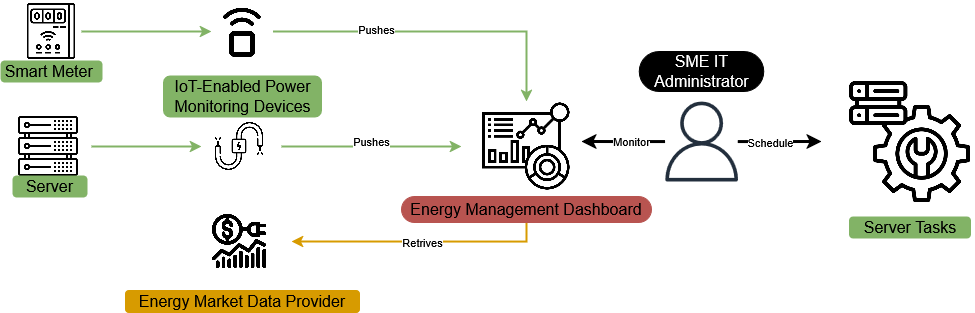
\includegraphics[width=0.8\textwidth]{fig/high_level_use_case.png}
    \caption{Overall Use Case of server admin using the energy management dashboard}
    \label{fig:highleveluse}
\end{figure}
Figure \ref{fig:highleveluse} illustrates the high-level use case, showing the actors and the flow of information. This approach enables SMEs to leverage real-time data and market signals to make informed decisions about server operations, ultimately reducing energy expenses and supporting sustainability goals.

\subsection{Prototype}
The prototype implements a serverless cloud architecture on Amazon Web Services (AWS) to collect,
process, and visualize energy data from multiple sources. Figure 1 illustrates the system
architecture and data flow of our proposedsolution.

\begin{figure}[htbp]
    \centering
    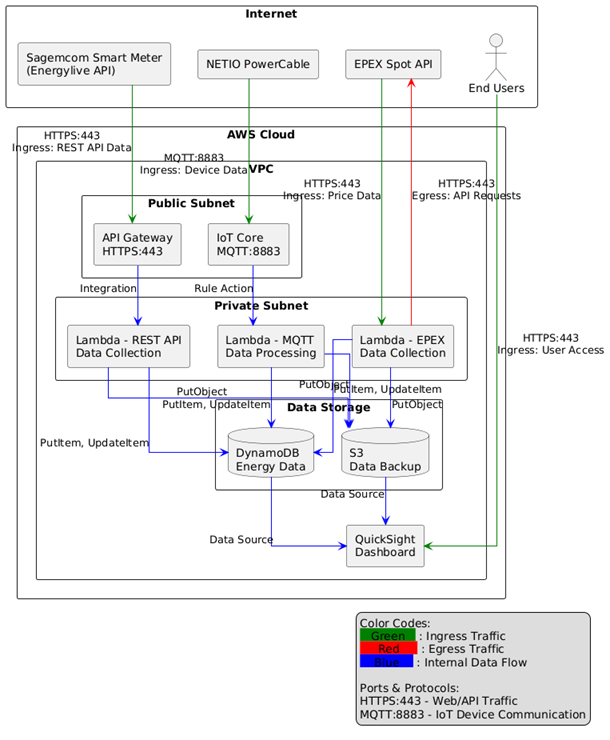
\includegraphics[width=0.6\textwidth]{fig/architecture2.png}
    \caption{System Architecture of the AWS implementation}
    \label{fig:architecture}
\end{figure}

The prototype consists of three main components that work together to deliver a comprehensive
energy monitoring solution for SME server environments. The data collection layer interfaces with
external devices and services to gather the necessary information. The data from the Sagemcom Smart
Meter is collectedvia the Energylive API, providing facility-level energy consumption data at
ten second intervals. This data includes overall electricity usage for the entire server room or IT
infrastructure. The NOUS A5T PowerCable device serves as an IoT sensor that measures power consumption
of individual servers and critical IT equipment, offering granular insights into which systems
contribute most significantly to the overall energy footprint. Additionally, the system integrates
with the EPEX Spot API to retrieve real-time and forecasted electricity market prices, which
are essential for cost optimization strategies.

The processing layer leverages AWS Lambda functions to handle the incoming data streams
efficiently. An API Gateway serves as the entry point for REST API requests from the Energy Live API,
ensuring secure and scalable communication. IoT Core manages MQTT connections from the NOUS A5T
PowerCable device, providing a reliable communication channel for this IoT sensor.
Three specialized Lambda functions handle different aspects of data processing: one dedicated to
REST API data collection from the Energy Live API, another processing MQTT messages from the IoT device
and a third specifically handling EPEX market data. This separation of concerns allows for
independent scaling and maintenance of each data processing pipeline while minimizing operational
overhead for SMEs with limited IT resources.

The storage and visualization layer ensures that data is both persistently stored and meaningfully
presented to SME operators. DynamoDB serves as the primary database, storing structured energy
consumption and pricing data in a format optimized for quick retrieval and analysis. S3 provides
backup storage and handles larger datasets that might be needed for long-term trend analysis. The
QuickSight service delivers interactive dashboards to end users, allowing them to explore their
server energy usage patterns, correlate consumption with pricing data, and identify optimization
opportunities through intuitive visualizations and reports that don't require specialized data
science expertise.

The architecture follows security best practices by implementing a Virtual Private Cloud (VPC) with
public and private subnets. External communications occur through secure protocols
(HTTPS for API traffic and MQTT over TLS for IoT devices), while internal data flows are restricted
within the VPC. This design ensures that sensitive consumption data remains protected while still
allowing for the necessary external integrations, addressing the security concerns that are
particularly important for SMEs handling sensitive business data.

\subsection{Evaluation Approach}
To evaluate the effectiveness of our approach, we will implement a comprehensive
evaluation approach that addresses technical performance, server energy
consumption patterns, and economic impacts. This multi-faceted evaluation will
provide insights into both the system's technical capabilities and its practical
utility for SME operators.

Server energy consumption analysis forms the core of our measurement approach.
Using the NOUS A5T PowerCable device, we will conduct detailed measurements of a
single server under various operational scenarios to establish energy consumption
profiles. Specifically, we will examine the following workloads (WL):

\begin{enumerate}[label=WL\arabic*]
    \item \textbf{Maximum computational load:} Simulation of 100\% CPU utilization across all
    cores using the stress-ng tool on a Linux virtual machine. The stress-ng
    command will be configured to spawn CPU-intensive worker processes equal to
    the number of available virtual CPUs, ensuring maximum load across all cores.
    This scenario represents peak computational demand typical of batch processing
    or intensive data analysis tasks. \cite{stressng2020}

    \item \textbf{I/O stress testing:} This WL conduct I/O stress testing to evaluate
    power consumption during intensive disk operations. Using fio (Flexible I/O Tester),
    we will simulate maximum Solid State Drive (SSD) utilization with sequential and random read/write
    patterns. This I/O-intensive scenario represents workloads common in database operations,
    log processing, and large file transfers, providing insights into storage
    subsystem energy requirements under heavy load.

    \item \textbf{System reboot cycle:} Measurement of the overall power consumption profile
    during a full reboot sequence of the host machine, capturing the energy
    requirements during shutdown, boot, and system initialization phases. This
    provides insights into the energy costs associated with maintenance operations
    and system updates.

    \item \textbf{Maintenance operations:} Monitoring of energy consumption during typical
    maintenance activities, specifically the patching process of a Linux virtual
    machine. This scenario represents regular administrative tasks that SMEs must
    perform to maintain security and system integrity.

    \item \textbf{Idle state:} Establishing the baseline energy consumption when the server is
    in an idle state with minimal active processes. This measurement is crucial
    for understanding the fixed energy costs of maintaining server availability
    even during periods of low utilization. \cite{moran2024dissecting,agilewatts2022}
\end{enumerate}

For each WL, the total energy usage consumption will be measured in kilowatt-hours (kWh) and power
consumption patterns over time, establishing detailed energy profiles that can be
correlated with specific operational states. These measurements will reveal the
energy intensity of different server activities and identify potential
optimization opportunities, such as scheduling high-consumption tasks during
periods of lower electricity pricing or implementing more efficient idle-state
management.
\newpage
To ensure reliable and representative measurements, each test scenario will be
conducted with specific time windows (TW):

\begin{enumerate}[label=TW\arabic*]
    \item For maximum computational load and I/O stress testing scenarios, each
    test window will span 30 minutes to capture steady-state behavior and account
    for any thermal effects or performance throttling that may occur during
    sustained high-load operations.

    \item System reboot cycle measurements will be conducted over multiple
    iterations, with each complete cycle (shutdown to fully operational)
    typically lasting 5-10 minutes, repeated 5 times to ensure consistency and
    account for variations in boot times.

    \item Maintenance operation measurements will cover the entire duration of
    typical update processes, estimated at 15-20 minutes per session, including
    download, installation, and post-update system stabilization periods.

    \item Idle state measurements will be conducted over longer 60-minute windows
    during off-peak hours to establish accurate baseline consumption patterns and
    capture any periodic background system activities.
\end{enumerate}

Each scenario will be repeated three times to ensure statistical validity and
account for any variations in system behavior or environmental conditions. A
minimum cool-down period of 10 minutes will be observed between test iterations
to ensure thermal conditions return to baseline.

